%!TEX encoding = UTF-8 Unicode
%!TEX root = ../lect-w10.tex

%%%


\Subsection{Veckans uppgifter}

\begin{Slide}{Veckans övning: \texttt{patterns}}
  Mål: Träna på matchning och undantag
\begin{itemize}
\item Uppg. 1--8: Matchning, \code{Option}
\item Uppg. 9--11: Undantag, \code{Try}
\item Uppg. 12: Laborationsförberedelse \code{Cell} och \code{Table}
\item Uppg. 13: Matchning eller dynamisk bindning?
\item Uppg. 14: avgöra likhet med matchning, \code{equals} utan arv
\item Uppg. 15--22: diverse fördjupningsuppgifter om matchning, undantag, hash-koder, likhet vid arvshierarki
\end{itemize}
\end{Slide}


\begin{Slide}{Veckans labb: \texttt{tabular}}\SlideFontTiny
%  \setlength{\leftmargini}{0pt}
\hspace{-2em}\begin{minipage}{0.7\textwidth}
\vspace{0.25em}
\Emph{Förberedelse:}
\begin{itemize}
\item Gör övning \code{patterns}, speciellt uppg. 12
\item Studera givna koden: {\SlideFontTiny \href{https://github.com/lunduniversity/introprog/tree/master/workspace/w10_tabular}{workspace/w10\_tabular}}
\item Fyll i denna enkät:
\\{\SlideFontTiny \url{https://goo.gl/forms/hC6JK2UQXVpbGECc2}}
\item Se svar här (snapshot uppdateras då och då): \url{http://cs.lth.se/pgk/favorit}
\end{itemize}

\Emph{Grunduppgift:}
\begin{itemize}
\item Terminalapp för hantering av kolumndata i textfiler.
\item Matchning används vid kommandotolkning.
\item \code{Option} används för inkapsling av ev. saknade värden
\item \code{Try} används för inkapsling av ev. undantag
\end{itemize}
\Emph{Extrauppgifter:} (Minst en)
\begin{itemize}
\item dialoger: \code{load}, \code{save}, kommando: \code{pie}, \code{bar}
\end{itemize}
\end{minipage}
\hfill\begin{minipage}{0.3\textwidth}
\centering
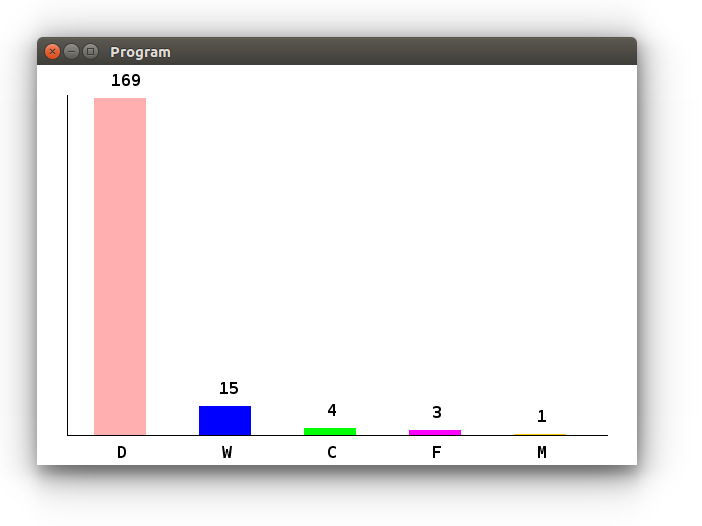
\includegraphics[width=0.95\textwidth]{../img/survey/bar}

\vspace{2em}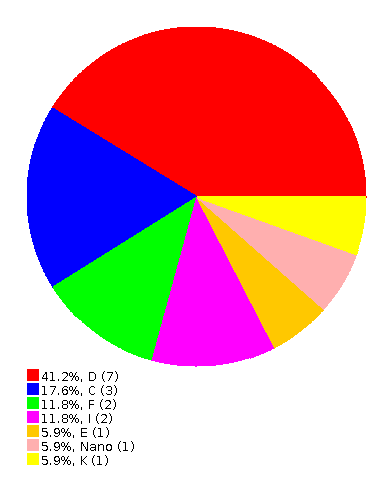
\includegraphics[width=0.7\textwidth]{../img/survey/pie}
\end{minipage}
\end{Slide}

\begin{Slide}{Extraundervisning del 3}
\begin{itemize}
\item  \Alert{Extraundervisning} i \Emph{E:1406} onsdag 21/11 kl 15:15-17:00
\item Hitta dit: \url{http://fileadmin.cs.lth.se/ehus/E1406.pdf}
\item Det finns gott om platser i den salen >70 platser så alla är välkomna
\item Fokus: grundläggande, långsam behandling på begäran, grumliga begrepp etc.
\end{itemize}
\end{Slide}


